\documentclass[]{article}

%Packages
\usepackage{hyperref}
\usepackage[margin=1in]{geometry}
\usepackage{setspace}

\usepackage{graphicx}
\usepackage[usenames, dvipsnames]{color}
\usepackage{setspace}
\usepackage{float}
\usepackage{fancyhdr}
\pagestyle{fancy}

%Package Settings
\onehalfspacing
\setlength\parindent{0pt}

\setlength{\parskip}{.5\baselineskip}   % Define spacing between two paragraphs

%opening
\title{DIME Dynamic Documentation Training \\ Stata Exercise}
\author{Luiza Andrade \& Mrijan Rimal}
\date{\today}

\makeatother

\fancyfoot{}
%\fancyhead[C]{\thepage}
\cfoot{\small{For the most recent version of the file, please check \url{https://github.com/worldbank/DIME-LaTeX-Templates/} } \\ \thepage}
\begin{document}

\makeatletter
\begin{titlepage}
	\begin{center}
		
\includegraphics[width=0.3\linewidth]{img/i2i.png}\\[10ex]
		{\LARGE \bfseries  \@title }\\[2ex] 
		{\Large  \@author}\\[20ex] 
		{\large \@date}
	\end{center}
\end{titlepage}
\makeatother

\section*{Introduction}
This exercise introduces you to how to export files from Stata that can be read in {\LaTeX}. See exercise 1 and 2 for instructions on how to import file into {\LaTeX}. After this exercise and exercise 1, you will have a document that is automatically updated each time you run your Stata and your {\LaTeX} code.

We have provided you with a do-file that has code that creates file that you can import in a {\LaTeX} document. We will go through these examples and then we will ask you to create some tables and graphs of your own using your own data. Note that this is not an exercise on Stata, only on exporting in {\LaTeX} format from Stata, so this exercise assumes knowledge of some intermediate level Stata commands.

\section*{Part 1: Setting up a Folder Structure}
Do not rush over this part. You will be forced to write an necessarily complicated {\LaTeX} code unless you set up a simple but well organized folder structure for where to export tables and figures from Stata. We strongly recommend that you start by setting up the following folder structure. 

Create one folder called \texttt{Output}, and inside this folder, create a folder called \texttt{Raw}. In the \texttt{Raw} folder you will export tables and graphs from Stata that you will import in your {\LaTeX} document. Your {\LaTeX} document will be saved in the \texttt{Output} folder.

See the example below. As your project grows bigger it is common that sub-folders are added in the \texttt{Raw} folder. For example, tables and figures often have separate folders. You will find your preferred way to organize this.

\begin{figure}[H]
	\centering
	
\includegraphics[width=0.6\linewidth]{img/outputRawFolders}
	\caption{Common Folder Structure}
	\label{fig:pathwin3}
\end{figure} 


\section*{Part 2: Setting your path for Stata}
We now need to tell all commands in Stata to save the tables and figures they export to the \texttt{Raw} folder. We want to create a global with the file path pointing to the \texttt{Raw} folder that we can use in our commands. Using a global instead of typing out the folder location in all commands both makes the code simpler, and makes it easier to update if you would have to move your folders.

Open the do-file \texttt{Export tables and images.do} that you find in the same folder as this handout. Look for the part that says:
\begin{center}
	\verb|global main_folder "<<<ENTER YOUR FOLDER PATH HERE>>>"|
\end{center}

You need to enter the path to the folder you created in part 1. If you have a Windows computer and you created your \texttt{Output} folder in your Documents folder, then your file path should look similar to this:
\begin{center}
	\verb|global main_folder "C:\Users\JoeSmith\Documents\Output"|
\end{center}

The following two sub-sections help you find the file path to the folder you just created if you are not sure how to do that. The first sub-section gives advice for Windows, and the second for Mac.

\subsection*{Finding Path on a Windows Computer}

Path to a file can be found by selecting a file and pressing {\color{red}SHIFT on your keyboard and RIGHT CLICKING your mouse and then clicking COPY AS PATH in the resulting drop down menu} as shown in Figure \ref{fig:pathwin3}.

\begin{figure}[H]
	\centering
	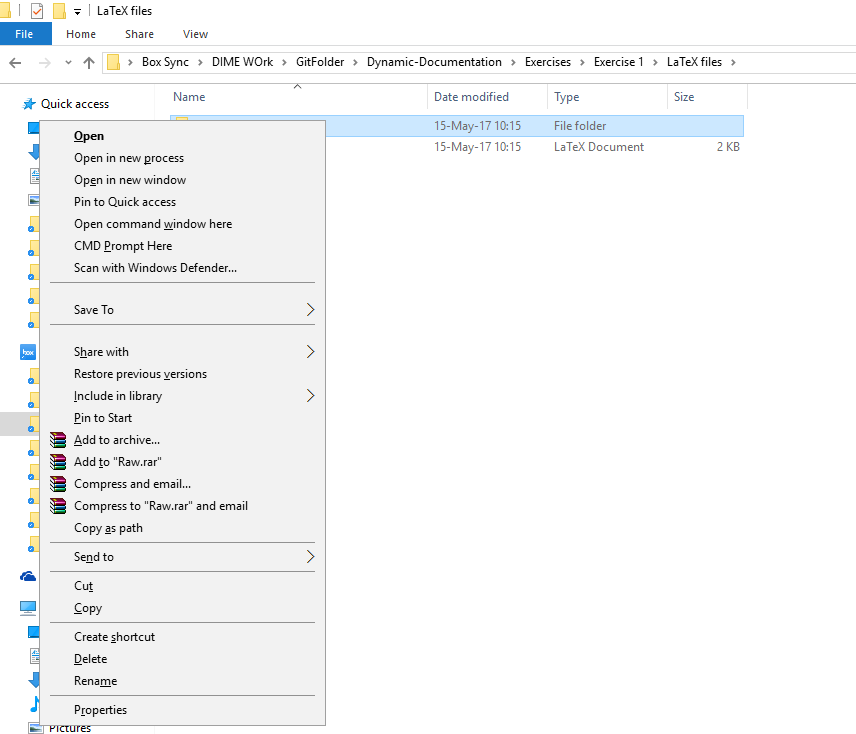
\includegraphics[width=0.9\linewidth]{img/pathwin3}
	\caption{Finding path on a Windows Computer - Solution 1}
	\label{fig:pathwin3}
\end{figure}


Another solution to finding the path on a Windows computer is shown in Annex 1.
	
\subsection*{Finding Path on a Mac}


\section*{Part 3: File Formats and Names}
Not all file formats that you can chose when exporting from Stata is valid to import into {\LaTeX}. Figures must be saved in \texttt{.png} format. All figures produced in Stata can be exported in \texttt{.png}. Even if some commands are not able to export in this format, you can use Stata to convert the figure for you. You will find more details on this in the parts below where we export figures. 

Tables must be saved in \texttt{.tex} format. Tables cannot be converted as easily as figures, so it is usually easier to find an alternative command that produces the same table but can export to \texttt{.tex} format. Most commands that export tables are able to export to this format so it should not be difficult to find an alternative.

Files exported in for example \texttt{MS Word} or \texttt{MS Excel} or in Stata's \texttt{.gph} format are not valid to import to {\LaTeX}.

Files exported from Stata should have a descriptive name. Otherwise you increase the risk for human errors, and the whole point of dynamic documents is to reduce exactly that. For example - rather than \texttt{graph1.png}, \texttt{graph2.tex}, names like \texttt{treatmentEffectGraph.png} would make it easier to understand what files we are using.

\section*{Part 4, Task 1: Tabulate Categorical Variables}

The code for this Part 4, 5 and 6, are all in the do file \texttt{Export tables and images.do}. The data that you will use is a sample data set that all instances of Stata alrady have. So you do not need a data file, the do-file will load this data set for you.

First we want to start with exporting a simple tabulate table of frequencies. We first use the command \texttt{tabulate} to generate the statistics, and use \texttt{esttab} to export it to \texttt{.tex} format. The command \texttt{estpost} that comes before the \texttt{tabulate} command takes the result for the tabulation and prepare them in a format that \texttt{esttab} can use. See the help files for \texttt{estpost} and \texttt{esttab} for more details on how this works. This is an exercise in {\LaTeX} and not the commands in the \texttt{estout} package so we will not go into more details about this at this point. 

To export the tabulation in \texttt{.tex} format using \texttt{esttab}, you simply set the file extension in the \texttt{using} option. Like this: \verb|using "$raw_output/categorical.tex", replace|. Remember to always have an explanatory file name.

Now check your \texttt{Raw} folder to see the \texttt{categorical.tex} file you have exported.

\section*{Part 4, Task 2: Regression table}

Similar to the previous task, we can use \texttt{esttab} to export regression tables. First we run the regressions we want to export the results for. The command \texttt{eststo:} before the regression commands stores the result of the regressions so that \texttt{esttab} can export all of them together. You can use any option to the regression that Stata allows. If Stata can run the regression and display the regression results in the Stata window, then \texttt{esttab} will be able to export those results to \texttt{.tex} format.

The difference between the two regressions is that the second regression includes fixed effects for region. We can use the command \texttt{estadd} to add text to the tables. In this example we use this to indicate which regression that included fixed effects. See the help files for \texttt{estout}, \texttt{estadd} and \texttt{esttab} for more details on how this works. This is an exercise in {\LaTeX} and not the commands in the \texttt{estout} package so we will not go into more details about this at this point. 

Similarly to the previous task, export the stored regression results using \texttt{esttab} to \texttt{.tex} format bys setting the file extenstion in the \texttt{using} option. Like this: \verb|using "$raw_output/regression_table.tex"|. \texttt{esttab} will export all results stored in your estimation memory. That is why it is important that we start each task with the code \texttt{estimates 	clear} in the do file. Otherwise we might add results from previous tables to this table.

Now check your \texttt{Raw} folder to see the \texttt{regression\_table.tex} file you have exported.

\section*{Part 5, Task 1: Manually Create a Graph and then Export it}

This task shows us how to export graphs created in Stata to export in a format that {\LaTeX} can read. Stata's save graph feature saves the graph in \texttt{.gph} format which only Stata can read. However, the \texttt{graph export} feature  saves the graph in a picture format i.e. png format which can be read by the photo viewer on your computer, phone and also {\LaTeX}. It is \emph{absolutely critical} to export the graph in this format, so that {\LaTeX} can import it. 

Using the \verb|graph export "$raw_output/regular_graph.png", width(5000) replace| 
exports the graph in png format which {\LaTeX} can read.

\textit{Note: This is different from the \texttt{iegraph} command where save can both export the graph in \texttt{.gph} and \texttt{.png} format. For Stata's \texttt{graph} command, export has be to be used to make it readable in {\LaTeX}}. 

Now check your \texttt{Raw} folder to see the \texttt{regular\_graph.png} file you have exported.

\section*{Part 5, Task 2: Using \texttt{iegraph} to create a figure}

While Stata's \texttt{graph twoway} uses the \texttt{save} feature to export pictures in a \texttt{.gph} format, and we have to use the \texttt{graph export} to export it in png format. Many commands, for example - \texttt{iegraph}, can export directly to either format using the same \texttt{save} option. 

This exercise teaches how to use \texttt{iegraph} to create a figure and export it to the graphs folder. On \texttt{iegraph}, while exporting a picture for {\LaTeX}, always make sure that the picture has the extension \texttt{.png} at the end of the filename. \textbf{Without that, \texttt{iegraph} is just going to export the picture in a format which only Stata can read!}

Using the \verb|save("$raw_output/iegraph.png")| ensures that the graphs are directly saved to the specified output folder. 

Now check your \texttt{Raw} folder to see the \texttt{iegraph.png} file you have exported.

\section*{Part 6: Making a Dynamic Document }

Here, we will produce a dynamic document. Please only do this do \textbf{if} you have completed up to \texttt{Part 5, Task 2} of the exercise. 

\begin{enumerate}
	\item Save the pdf created upto now in a separate location from your \texttt{.tex} file.
	\item Go to \texttt{line 60} of the Stata do file and change the seed from \texttt{215320} to a number different than \texttt{215320}.\\ \textit{Note: Changing seeds is not recommended for actual projects. The change in seeds here is used to highlight the change in treatment/control groups.}
	\item Rerun the do-file with the new seed.
	\item Now, open the earlier created {\LaTeX} file and press \textit{Build and Compile} under the \textit{Tools}.
	\item Now if you compare the pdf file you have just generated with the one you saved earlier, you will find that the tables would have updated automatically. 
\end{enumerate}

\section*{Part 7, Using a do-file to edit a .tex file after exporting it}
During this part of the exercise, you will learn how to use commands in Stata to format your tables. While tables exported from Stata to {\LaTeX} are generally very nice, sometimes they need to be tweaked a little to make them look nicer. So, in this exercise, you'll use the \texttt{filefilter} command in Stata to make small changes to the files exported by Stata. 

\newpage
\section*{Annex 1} {\label{annex1}}

\begin{figure}[H]
	\centering
	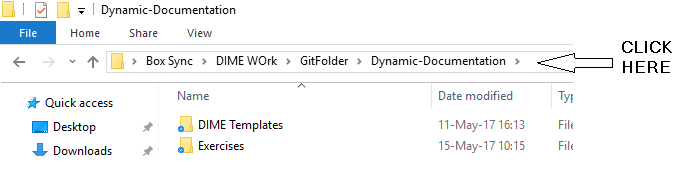
\includegraphics[width=1\linewidth]{img/pathwin}
	\caption{Finding Path on a Windows Computer}
	\label{fig:pathwin}
\end{figure}
As shown in Figure \ref{fig:pathwin}, left clicking(normal click) on the bar at the top of the \texttt{File Explorer} windows where our files are saved shows us the complete path to the files in a Windows computer. \\

\begin{figure}[H]
	\centering
	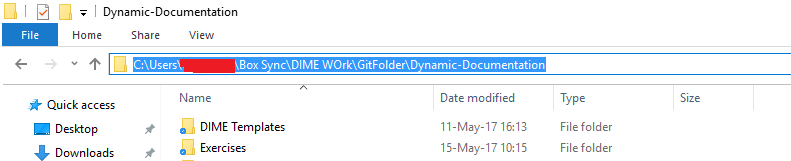
\includegraphics[width=1\linewidth]{img/pathwin2}
	\caption{Path shown on a Windows Computer}
	\label{fig:pathwin2}
\end{figure}

We can see in Figure \ref{fig:pathwin2}, that the complete path to the folder is shown. We can then paste this path when setting the path in our Stata do-file and changing the path where it says \begin{verbatim}
global main_folder ``<<<ENTER YOUR FOLDER PATH HERE>>>''
\end{verbatim} 
	
\end{document}
